\pagebreak
\pagenumbering{arabic}
\chapter{Theoretical Background}

\section{Introduction}

The significance of the sense of vision for humans, in our contemporary everyday lives as well as in our evolution as a species, cannot be understated. While there is no clear consensus that vision is our most important sense, since that is dependent on one's cultural, societal and technological influences, there exists a large body of data drawn from cross-sectional observational research and surveys, as well as expert opinion of practitioners and researchers that leans towards the fact that vision is considered the most valued sense to the public.

Since prehistoric times, it is our vision that has aided us in our survival, by means of allowing us to advantageously select healthy mates, forage ripe fruit against a green foliage and detect predators through their natural camouflage, just to name a few benefits. Even in today's world, the majority of the information we process hails from our eyesight, whether it originates from the environment or from a computer screen.

However controversial the topic of the superiority of vision over our other senses might be, what is truly undebatable is that our evolution and eventual dominance as a species has been a consequence of the capabilities of our brain. It is the current form of the human brain after all, displaying an astonishingly intricate way in which it processes visual stimuli, that was preferentially chosen through natural selection to translate visual information to fit the species' best interests. Thus, it could be argued that to achieve a holistic understanding of the sense of vision, we need to delve into the patterns of activation induced in the brain by visual stimulation.

\section{Visual Information Flow In The Brain}

Light entering the eye creates a cascade of neuronal events throughout the optic pathway, which describes the anatomical pathway by which electrical signals generated by the retina are sent to the brain.

\subsection{The Optic Pathway}

The optic pathway begins in the retina, which is a complex structure made up of ten different layers. Notably, the photoreceptor layers consist of the rods and cones, which generate action potentials with the help of rhodopsin through photosensitive cycles. The ganglion cell layer and nerve fiber layer serve as the foundation of the optic nerve; the former contains the cell bodies, and the latter contains the axons as they stream across the retina. The nerve is surrounded by the dura, which is a continuation of that of the brain, allowing free movement of \gls{CSF} between the eye and the intracranial vault. The axons exit the orbital part of the optic nerve through the orbital foramen, simultaneously with the ophthalmic artery and sympathetic fibers.

\clearpage %potentially replace with \vspace after text is set in stone.

\begin{wrapfigure}{l}{0.42\textwidth}
	\centering
	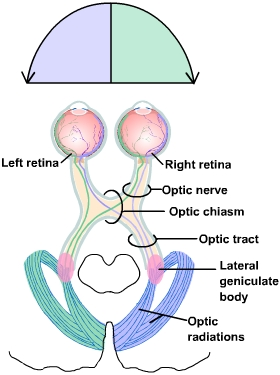
\includegraphics[width = 0.42\textwidth]{assets/images/Optic_Pathway.jpg}
	\caption[The Visual Pathway]{Illustation of the Visual Pathway and its components, including the course of information flow from the right (green) and left (blue) hemifields of the two eyes' visual fields. Adapted from page \cite{optic_nerve}.}
	\label{fig:OpticPath}
\end{wrapfigure}

They then enter the optic canal, a bone-encased tunnel intended to protect the nerve, exit into the middle cranial fossa to form the intracranial part of the optic nerve, which continues till the two optic nerves join together to form the optic chiasm directly behind and above the pituitary stalk. Beyond the chiasm, the pathway continues as two distinct tracts, each carrying the temporal fibers from the other eye. The optic tract then passes posteriorly where most of the axons synapse in the layers of the \gls{LGB} of the midbrain, which is a posterolateral extension of the thalamus.

The majority of the fibers pass posteriorly to become the genico-calcarine tracts, which have both parietal and temporal loops and terminate into the cuneus gyrus and lingual gyrus of the primary visual cortex, respectively (see \autoref{fig:OpticPath}). Perception of sight ultimately derives from processing within this and adjacent areas of the brain \cite{Gupta2022}.

\subsection{Information Processing In The Visual Cortex}

\begin{wrapfigure}{l}{0.29\textwidth}
	\centering
	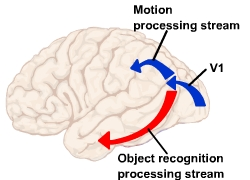
\includegraphics[width = 0.29\textwidth]{assets/images/Info_distinction_from_vis_cortex.jpg}
	\caption[Visual Information Flow Bifurcation]{Distinction in the flow of visual information from the \gls{V1} to other cortical areas. The ventral stream transfers information to the inferior cortical areas, whereas the dorsal stream tranfers it to the more superior cortex. Adapted from page \cite{optic_nerve}. }
	\label{fig:processing_streams}
\end{wrapfigure}

The modules that compose the visual pathway from the retina to higher visual centers follow two diverging streams in the cortex: one pathway extends dorsally to terminate within the parietal lobe, including the motion detection area, \gls{MT}, and the visual areas of the posterior parietal cortex; the other pathway extends ventrally to terminate in the temporal lobe, including \gls{V4} and \gls{IT}. It is suggested \cite{Mishkin1983} that these two pathways serve different functions: the dorsal pathway is concerned with \textit{where} an object is in visual space (motion, distance); the ventral pathway is concerned with \textit{what} an object is (form, color, texture, all of which are involved in object recognition) (see \autoref{fig:processing_streams}).

The \gls{V1} area of the brain is involved in the initial cortical processing of all visual information necessary for visual perception. The color, shape and movement information from the thalamus are sent to different neurons within \gls{V1} for further processing and then sent onto different areas of the extrastriate visual cortex. 

Within \gls{V1}, information processed by \gls{blob cells} is used in color perception, color discrimination and the learning and memory of the color of objects. The \gls{blob cells} are the "color" processing cells of the \gls{V1}. On the other hand, \gls{V1} \gls{interblob cells} belong in one of two categories: The first are location specific cells, which respond best when the stimulus is in a specific location of the receptive field. The information processed by these cells is used in object perception, discrimination, learning and memory, or in spatial orientation. These cells are the "shape, form and location" cells of the \gls{V1}; The second kind of \gls{interblob cells} is the movement sensitive ones, which respond best to moving stimuli and are utilized to detect object movement, direction and velocity and to guide eye movements. These are the "motion detecting" cells of \gls{V1}.

The \gls{V1} sends input to the extrastriate visual cortex, which includes all the occipital lobe areas surrounding the \gls{V1}. The extrastriate cortex in non-human primates has been subdivided into as many as three functional areas, \gls{V2}, \gls{V3} and \gls{V4}. The information corresponding to each of the aforementioned categories of neurons in the \gls{V1} is sent  to different areas of the extrastriate visual cortex.

Specifically, the neurons in the inferior temporal visual association cortex, i.e., the ventrally located neurons accessed by the ventral stream, are responsible for processing information necessary for our abilities to recognize objects and colors, read text and learn and remember visual objects. It can thus be concluded that, in the context of this thesis, which investigates task-evoked visual stimulation, this area of the brain will be the region of interest. More deliberately, four regions of extrastriate cortex are of utmost importance for the purposes of this current dissertation: the \gls{FFA}, the \gls{PPA}, the \gls{LOC} and the \gls{EBA}.

\subsection{Category-Specific Information Processing Areas In The Extrastriate Visual Cortex}

% FFA Description
In the early 1990s, \gls{PET} demonstrated activation of the ventral visual pathway, especially the \gls{FG}, in a variety of face perception tasks \cite{Haxby1991, Sergent1992}. \gls{fMRI} studies of the specificity of these cortical regions for faces began with demonstrations of fusiform regions that responded more strongly to faces than to letter strings and textures \cite{Puce1996}, flowers \cite{McCarthy1997} and other mixed stimuli  \cite{Kanwisher1997}. Although face-specific \gls{fMRI} activations could also be seen in many subjects in the region of the \gls{fSTS} and in the occipital lobe in a region named the \gls{OFA}, the most consistent and robust face-selective activation was located on the lateral side of the mid-fusiform gyrus, within the \gls{IT}, in a region consequently named the \gls{FFA}. With the methods currently used, this region can be functionally identified in almost every normal subject in a short "localizer" \gls{fMRI} scan contrasting the response to faces versus objects \cite{Kanwisher2006}.

% PPA Description
Another well studied category-selective region of cortex is the \gls{PPA}, responding strongly to a wide variety of stimuli depicting places and/or scenes (e.g. outdoor and indoor scenes and houses) compared to various control stimuli such as faces or scrambled scenes \cite{Epstein1998}. Additionally, it has been found that \gls{PPA} activity is not affected by the subject's familiarity with the place depicted, does not increase when subjects experience a sense of motion through the scene, and is greater when viewing novel versus repeated images \cite{Epstein1999}. Using sets of scenes that had viewpoint changes, it was demonstrated that the \gls{PPA} treated scenes with viewpoint changes as different \cite{Epstein2003}, suggesting that this area represents scenes as individual snapshots of each view rather than as a broader scene that integrates multiple similar snapshots. However, when subjects saw different snapshot views from panoramic scenes, which represented clearly different views but appeared to come from the same scene, \gls{fMRI} showed no attenuation for panoramic repeats in the \gls{PPA}, suggesting viewpoint-specificity \cite{Park2009}.

% LOC Description
The \gls{LOC} is located on the lateral bank of the \gls{FG}, extending both ventrally and dorsally, consisting of the \gls{MOG} and the \gls{IOG} as well as the \gls{LOS} between them. This region has been shown to respond more strongly when subjects passively view photographs of common everyday objects than when they view visual textures without obvious shape interpretations \cite{Malach1995}. Importantly, the magnitude of the response was no different for familiar objects and unfamiliar ones with clear three-dimensional shape interpretations (e.g. Henry Moore sculptures). A similar result was found using line drawings \cite{Kanwisher1996}: stronger responses to three-dimensional objects depicted in line drawings, whether familiar or novel, compared to scrambled line drawings. Several more studies provide evidence that the entire \gls{LOC} region responds more strongly to intact objects with clear shape interpretations, than to control stimuli that do not depict clear shapes \cite{Kalanit1998, Murtha1999, Kalanit2001}.

% EBA Description
Since the turn of the twentieth century, neuroimaging studies have identified two brain regions of the extrastriate visual cortex that are highly sensitive to the perception of human bodies and body parts in comparison to other classes of stimuli. These regions are the \gls{EBA}, which is a body-selective focal region located partly at  both the posterior inferior temporal sulcus and the middle temporal gyrus \cite{Downing2001} and the \gls{FBA} found ventrally in the fusiform gyrus \cite{Peelen2005}. Evidence derived from \gls{fMRI} studies has shown that both areas become significantly activated in response to body and body parts stimuli visually presented in different formats such as photos, line drawings, stick figures and silhouettes compared to control stimuli like faces, tools and scenes \cite{Spiridon2006, Weiner2010, Amoruso2011}. Additionally, research seems to suggest that the \gls{EBA} also participates in more complex functions like body discrimination of self versus others. \cite{Pann2021}. It has been suggested that \gls{EBA} and \gls{FBA} can be functionally dissociated, with a more selective activation for local body parts in \gls{EBA} relative to more holistic images of the human body in \gls{FBA} \cite{Taylor2007}.

\begin{figure}[htbp]
 	\centering
	\begin{subfigure}{0.49\textwidth}
		\centering
		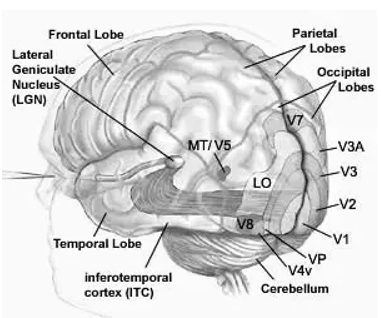
\includegraphics[width = 0.8\textwidth, height = 4cm]{assets/images/visual_areas.png}
		\caption{Graphic of the visual areas of the brain thought to be geographically within the occipital lobe \cite{visual_centers}. Adapted from \paper{Perez}{Perez2012}.}
		\label{fig:Visual_areas}
	\end{subfigure}
	\hfill
	\begin{subfigure}{0.49\textwidth}
		\centering
	 	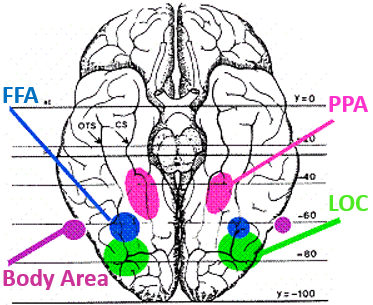
\includegraphics[width = 0.8\textwidth, height = 4cm]{assets/images/brain_areas.png}
		\caption{Brain diagram including some category-specific information processing areas of the brain \cite{prosopagnosia}. Adapted from page \cite{brain_areas}.}
		\label{fig:Specific_areas}
	\end{subfigure}
	\caption[Brain Regions of Interest]{Illustration of \gls{ROIs} in the human brain.}
 	\label{fig:Brain_Areas}
\end{figure}

% Mutual exclusivity of category specific areas
While it has been clearly established that certain areas of the extrastriate visual cortex process category-specific information (see \autoref{fig:Brain_Areas}), another critical inquiry, particularly in the context of \gls{fMRI} \gls{MVPA} of contrasts among different classes of stimuli, is whether each region is exclusively selective for target-specific stimuli or if there is overlap between regions, especially considering the close proximity among them. One such case is the \gls{FFA} and \gls{FBA}, which have been found in many subjects to be adjacent or overlap with one another. However, in \gls{ROIs} that omit overlapping voxels it has been demonstrated \cite{Schwarzlose2005} that, \gls{FFA} showed no response above control objects for body stimuli and \gls{FBA} showed no response above control objects for face stimuli, confirming strong selectivities in distinct but adjacent regions in the \gls{FG}. Similar conclusions of high selectivity have been reached \cite{Mengjin2022} in regard to the \gls{FFA} and the \gls{PPA}, where results revealed distinct response properties between the two regions for faces and houses respectively, implying a combination of spatially discrete domain-specific and relatively distributed domain-general organization mapping in the human ventral temporal cortex.

% Neuroimaging techniques intro and segway into fMRI explanation
Many brain imaging tools are available to cognitive neuroscientists, including \gls{PET}, \gls{NIRS}, \gls{MEG}, \gls{EEG} and \gls{fMRI} \cite{Xue2010}. Some of those have had their time in the spotlight in the previous decades but have now been overshadowed by the more advanced, non-invasive neuroimaging techniques such as \gls{EEG} and \gls{fMRI}, which allow researchers to directly observe brain activities while subjects perform various perceptual, motor or cognitive tasks. It is therefore imperative that we acquire at least a basic understanding of the procedures and metrics through which these techniques work if we are to be able to interpret their results and further analyze them. For the purposes of this paper, we focus on the inner workings of \gls{fMRI}, which is the instrument used to extract the data used in our \gls{MVPA}.

\section{Mechanisms of Functional Magnetic Resonance Imaging}

\subsection{Fundamentals of NMR Signal Generation}

% Summary of NMR signal generation
The outline of the process by which \gls{fMRI} signal is generated begins with the scanner creating a powerful magnetic field  \( \vec{\boldsymbol{B_0}} \). All magnetic moments of nuclei with nonzero spin, including protons which are found overwhelmingly in the form of hydrogen nuclei in the human brain, tend to weakly align with \( \vec{B_0} \), creating a net macroscopic magnetization \( \vec{\boldsymbol{M_0}} \). A coil within the machine, then transmits a \gls{RF} transverse magnetic field at the resonant frequency \text{\( \omega_0 = \gamma \cdot B_0 \)}, where \( \boldsymbol{\gamma} \) is the \gls{gyromagnetic ratio}, tipping the magnetic moment from alignment and causing it to precess around the \( \vec{B_0} \) axis at angular frequency \( \boldsymbol{\omega_0} \). For protons, \text{\( \gamma = \ \SI{2.675e8}{\radian \per \tesla} \)} and at a typical magnetic field strength of \SI{3}{\tesla}, the precession frequency \text{\( \nu_0 = \omega_0 / 2\pi \)} is approximately \SI{128}{\mega\hertz}. Following this interaction, the net magnetization vector can be described as two components: the remaining longitudinal magnetization along the \( \vec{B_0} \) axis; and the rotating transverse magnetization perpendicular to \( \vec{B_0} \). The rotating component generates an oscillating magnetic field that induces a current in a nearby coil, thereby producing the basic measured \gls{NMR} signal. Over time, the transverse magnetization decays exponentially with a characteristic time constant \( \boldsymbol{T_2} \), and the longitudinal magnetization recovers exponentially towards its equilibrium value \( M_0 \) with a time constant \( \boldsymbol{T_1} \) \cite{Buxton2013, Suriaga2009}.

\subsection{Relaxation Time Constants}

% T1
T1 relaxation is the process by which the $z$ component of the net magnetization $M$ returns to its initial maximum value $M_0$ parallel to $B_0$. It can be modeled as a simple exponential with $T1$ as a first-order time constant, defining it as the time required for $M_z$ to reach $(1 - \frac{1}{e})$ or about $63\%$ of its maximum value (see \autoref{fig:T1} \cite{T1}). A typical value for $T1$, inside a \SI{3}{\tesla} magnetic field, in gray matter of the human brain is about $\SI{1.0}{\second}$. As $M_z$ grows toward $M_0$ the energy of the spin system decreases, considering that more spins statistically favor the spin-up parallel orientation, which is the lower of the two potential energy states. Consequently, as T1 relaxation occurs, energy dissipates from the system in the form of heat, hence the synonym for T1 relaxation, "thermal relaxation". This heat is then transferred to nearby nuclei via collisions, rotations, or electromagnetic interactions, and becomes unrecoverable. At its core, T1 relaxation represents an energy exchange process between spins and their external environment.

Blood inflow and \gls{CBF} can act to decrease the T1 values of blood and extravascular tissue components, resulting in a modified, measured T1 constant, termed T1*. Flowing blood moves spins from outside the imaging plane into the slice pixels. When spins in the imaging plane are saturated, signal from the unsaturated inflowing blood is enhanced relative to the surrounding stationary spins. The magnitude of this inflow contribution in vessels depends on the \gls{MRI} parameters, \gls{TR} and \gls{flip angle} $\theta$. When the \gls{TR} is sufficiently long to allow arterial blood spins from outside the imaging slice to flow into capillaries and exchange with extravascular tissue water, spatially specific perfusion contrast appears. In the extravascular tissue pool, \scalebox{1.2}{$\frac{1}{T_1^*} = \frac{1}{T_1} + \frac{f}{\lambda}$} where $f$ is the \gls{CBF} and $\lambda$ is the blood-to-tissue partition coefficient \cite{Detre1992}. 

\begin{figure}[htbp]
    \centering
    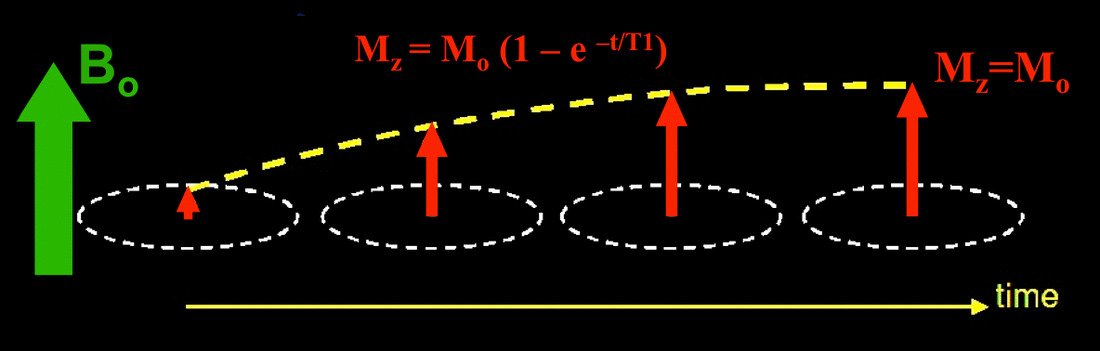
\includegraphics[width = 0.75\textwidth]{assets/images/T1_illustration.jpg}
    \caption[T1 Relaxation]{Illustration of T1 relaxation. Adapted from page \cite{T1}.}
    \label{fig:T1}
\end{figure}

% T2
T2 is the time constant for decay or dephasing of transverse magnetization $M_{\text{xy}}$ and may occur with or without energy transfer. T2 relaxation is considered to follow first order kinetics, resulting in a simple exponential decay (identical to radioactive decay), resulting in T2 being the time required for the net transverse magnetization to fall to $\frac{1}{e}$ or approximately $37\%$ of its initial value \cite{T2}. Following a $90^\circ$ \gls{RF} pulse, the initial Boltzman distribution of spins in the $z$ direction, constituting $M_z$, is preserved and transformed by the rotation into what is termed "phase coherence" in the $\text{xy}$ plane, in the form of an asymmetrical clustering of spins which gives rise to a net transverse magnetization $M_{\text{xy}}$. After the pulse is over, the many transverse spin components will precess within the plane at the Larmor frequency. The presence of a non-zero $M_{\text{xy}}$ at any time, is evidence of persistent asymmetry of transverse components of angular momentum. Any process that disrupts either the number or the relative positions of said components will result in T2 relaxation. These fall into one of two general categories.

The first kind of T2 relaxation is when it accompanies T1 relaxation. If energy radiated during the latter, were to affect one of the spins contributing to $M_{\text{xy}}$, both its angular momentum components would be randomly changed, and it would immediately lose phase relations with other spins, thus it would stop contributing to $M_{\text{xy}}$ altogether. As a result, $M_{xy}$ would be diminished, meaning T2 relaxation would have occurred. We can conclude that any process causing T1 relaxation also results in T2 relaxation, while the opposite is not true. This is sometimes called the T1 contribution to T2 and explains why T1 needs to be monitored as well, even though it is the sweep of the transverse magnetization alone that induces a current in the receiver coils, ultimately producing the \gls{NMR} signal.

On the contrary, stand-alone T2 relaxation is referred to as the secular contribution to T2. One of the most common ways for this to occur is when a spin is situated in a molecular environment where it experiences a local static magnetic field disturbance \( B_{\text{loc}} \) in addition to \( B_0 \). The component \( B_{\text{loc}-z} \) of the secondary magnetic field, parallel to the main field, is added to the total magnetic field experienced by the spin, causing it to precess at a frequency \text{\( \omega_0^{\prime} = \gamma \cdot (B_0 + B_{\text{loc}-z}) \)}. Meanwhile, the unaffected spins continue to precess at the original Larmor frequency. Over time, a phase difference of \( \phi = \gamma \cdot B_{\text{loc}-z} \cdot t \) develops between the disturbed spin and the rest, leading to loss of phase coherence, T2 relaxation, and reduction in \( M_{\text{xy}} \). Secular T2 relaxation can also occur due to a special dipolar interaction, where a pair of spins simultaneously exchange their longitudinal angular momentum components, resulting in no net T1 effect but loss of T2 coherence. In gray matter in the human brain, at a field strength of 3 \si{\tesla}, measured T2 is around \( \SI{0.1}{\second} \).

\begin{figure}[htbp]
    \centering
    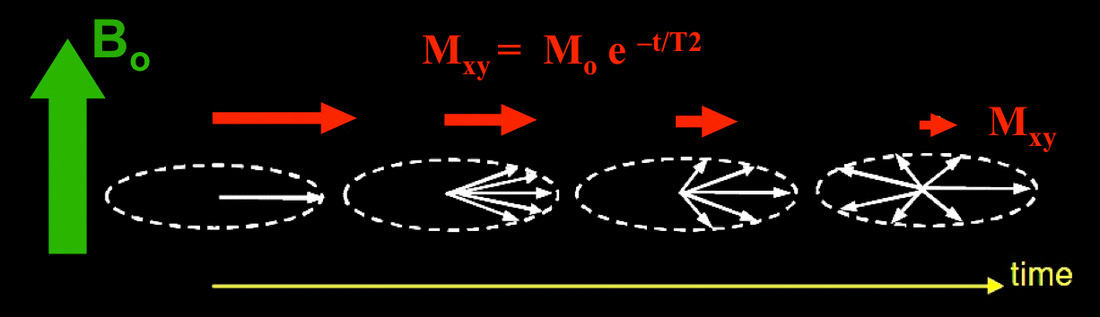
\includegraphics[width = 0.75\textwidth]{assets/images/T2_illustration.jpg}
    \caption[T2 Relaxation]{Illustration of T2 relaxation. Adapted from page \cite{T2}.}
    \label{fig:T2}
\end{figure}

% T2*
It needs to be noted that in any real \gls{NMR} experiment, the transverse magnetization decays much faster than would be predicted by natural atomic and molecular mechanisms; this faster rate is denoted \textbf{T2*}. It can be considered as "observed" or "effective" T2, whereas the latter can be thought of as the natural T2 of the tissue being imaged. T2* is always less than or equal to T2 (see \autoref{fig:T2_star}). T2* results principally from inhomogeneities in the main magnetic field, which may arise from intrinsic defects in the magnet itself or susceptibility-induced field distortions caused by tissue or other materials within the field. Certain \gls{MR} sequences using gradient echoes and relatively long \gls{TE} values are called \gls{T2w} \cite{T2_star}.

% Mathematics of NMR signal
Pixel sizes in typical \gls{fMRI} studies are a few millimeters; each pixel may therefore include blood, extravascular tissue, and \gls{CSF}. Since arterial blood and venous blood have different T2 values, these should be considered separately, with the assumption that capillary content is partly arterial blood and partly venous blood. Thus, \gls{NMR} signal intensity from a pixel is the sum of signals originating from multiple compartments with different spin density and relaxation parameters. The \gls{fMRI} intensity $S$ can be described as seen in \autoref{eq:MRI_Signal_Intensity} \cite{Kim2012}.

\begin{equation}
	\label{eq:MRI_Signal_Intensity}
	S = \sum_i \rho_i \times V_i \times M_{\text{ss},i} \times e^{-\text{TE}/T_{2,i}^*}
\end{equation}

\begin{equation}
	\label{eq:ss_magnetization}
	\displaystyle M_{\text{ss},i} = \frac{\left(1 - e^{-\text{TR}/T_1^*}\right) \sin\theta}{1 - \cos\theta \times e^{-\text{TR}/T_1^*}}
\end{equation}

Subscripts \( i \) indicate each compartment; \( \rho \) is the water proton spin density, directly related to water content in the tissue; \( V \) is the volume fraction, which is approximately \( 1\% \) for arterial blood \cite{Ito2001} and \( 2.5 \text{-} 3\% \) for venous blood \cite{An2002a, An2002b}; \( M_{\text{ss}} \) is the steady-state magnetization given by \autoref{eq:ss_magnetization}; \( \textit{\gls{TR}} \) is the repetition time; \( T_1^* \) is the apparent longitudinal relaxation time in the presence of inflow; and \( \theta \) is the \gls{flip angle}. It should now be evident that \gls{fMRI} signal changes depend not only on imaging parameters, but also on biophysical responses that significantly affect these variables.

\begin{figure}[htbp]
    \centering
    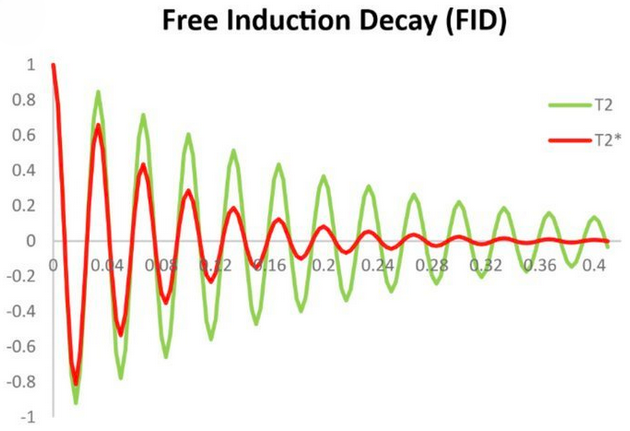
\includegraphics[width = 0.75\textwidth]{assets/images/FID.png}
    \caption[NMR Signal]{The observable \gls{NMR} signal generated by non-equilibrium nuclear spin magnetization precessing about $B_0$. Adapted from page \cite{T2_star_graph}.}
    \label{fig:T2_star}
\end{figure}

% fMRI Techniques and segway into BOLD
At this point, with a solid grasp of the general physical quantities involved in the production of \gls{NMR} signals, it is important to link these quantities with biological processes in the human brain to progress from pure anatomical imaging to functional display. Several techniques can detect changes in metabolic activity following neural activation, including contrast \gls{fMRI}, \gls{BOLD} \gls{fMRI}, and perfusion \gls{fMRI}. Contrast \gls{fMRI} requires the injection of contrast agents such as iron oxide coated with sugar or starch. Although this method can provide relatively strong signals, researchers are often reluctant to use this semi-invasive method with healthy volunteers. Perfusion \gls{fMRI} utilizes \gls{ASL} to magnetically label hydrogen nuclei in arterial blood and then images their distribution in the brain. The signal received from this technique is more stable and less noisy than that of \gls{BOLD} \gls{fMRI}, but it is also relatively weak, and the length of image acquisition time makes it impractical for many applications. Currently, the most widely used \gls{fMRI} method is \gls{BOLD} imaging.

\subsection{Blood Oxygen Level Dependent \textit{(BOLD)} Signal}

% Short abstract of subsection.
The \gls{BOLD} signal, captured in \gls{fMRI} detects changes in \gls{HbR} driven by localized changes in brain blood flow and blood oxygenation, which are coupled to underlying neuronal activity by a process termed neurovascular coupling. \gls{fMRI} relies upon the measurement of T2* relaxation, which is sensitive primarily to local concentrations of paramagnetic \gls{HbR} in venous blood, rendering the latter a naturally occurring contrast agent. Interpretation of the \gls{fMRI} \gls{BOLD} signal is intrinsically linked to understanding the underlying physiological and metabolic processes in the brain that modulate blood flow.

% How BOLD manifests.
The \gls{BOLD} effect related to neural activity arises because of two distinct phenomena. The first is that when \gls{Hb}-the molecule in blood that carries oxygen-lose the oxygen to become \gls{HbR}, its magnetic properties change in a subtle way: \gls{HbR} is paramagnetic, and alters the magnetic susceptibility of blood, whereas \gls{HbO} and the surrounding tissue \ce{H2O} are diamagnetic (see \autoref{fig:HbMagnetic}). The difference in susceptibility between blood vessels and the surrounding tissue creates local magnetic field distortions that decrease the net \gls{MR} signal. In the brain, a typical \gls{OEF}-the fraction of \ce{O2} carried by an element of blood that is removed in passing through the capillary bed-is approximately 40\% and in a 3 T magnetic field this level of \gls{HbR} in the veins and capillaries is sufficient to reduce the \gls{MR} signal by about 10\% in the baseline state, compared to what it would be if no \gls{HbR} was present. 

\begin{wrapfigure}{l}{0.4\textwidth}
   \centering
   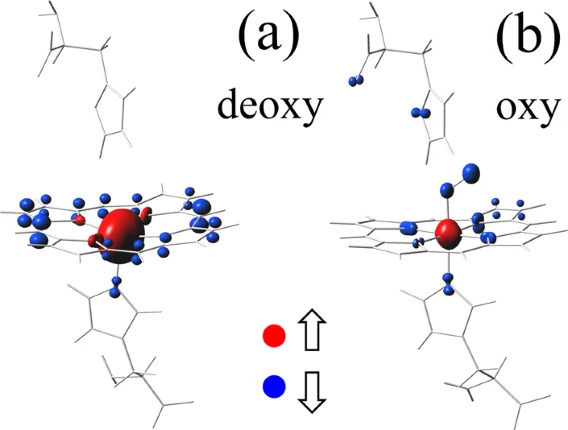
\includegraphics[width = 0.4\textwidth, height = 4.5cm]{assets/images/DeoxyHb_magnetic.jpg}
   \caption[Oxy- and Deoxy-hemoglobin Magnetic Moment Density]{Illustation of magnetic-moment density \textbf{M(r)} for the \textbf{(a)} \gls{HbR} and \textbf{(b)} \gls{HbO} heme clusters at \textit{T = 150K}. The magnitude of \textbf{M(r)} at an atomic site is proportional to the volume of the bubble at that site. Adapted from Fig. 2 p.2 \paper{Mayda}{Mayda2020}.}
   \label{fig:HbMagnetic}
\end{wrapfigure}

The combination of the aforementioned with the biophysical phenomenon, that when a brain area is activated, the blood flow increases-via a process called the hemodynamic response-to a greater degree than the oxygen metabolic rate, produces a useful basis for an experimental signal acquisition technique. The second phenomenon leads to a reduction in the \gls{OEF}, a seemingly paradoxical scenario in which the venous blood is more oxygenated, despite the increase in oxygen metabolic rate, because the blood flow has increased to a greater extent. Taken together, these two phenomena produce the \gls{BOLD} effect, a local increase in the \gls{MR} signal due to a reduction in the \gls{OEF} during increased neural activity. \cite{Buxton2013}

% Misconception tackled.
A prevailing misconception is that \gls{BOLD} provides a direct measurement of neuronal oxygen consumption. However, this is generally not the case; classic positive \gls{BOLD} signals, seen in response to functional stimuli, represent a decrease in \gls{HbR} and thus an overoxygenation of the responding region \cite{Attwell2002}. These positive \gls{BOLD} responses correspond to a local, actively actuated, increase in blood flow and volume, which brings blood in sufficient excess to increase local oxygenation levels \cite{Raichle1998}. This response typically begins within about 500ms and peaks 3 to 5 seconds after stimulus onset \autoref{fig:BOLD}, even for short stimuli lasting less than 1 second, with more complex dynamics for prolonged stimuli.

\begin{figure}[htbp]
    \centering
    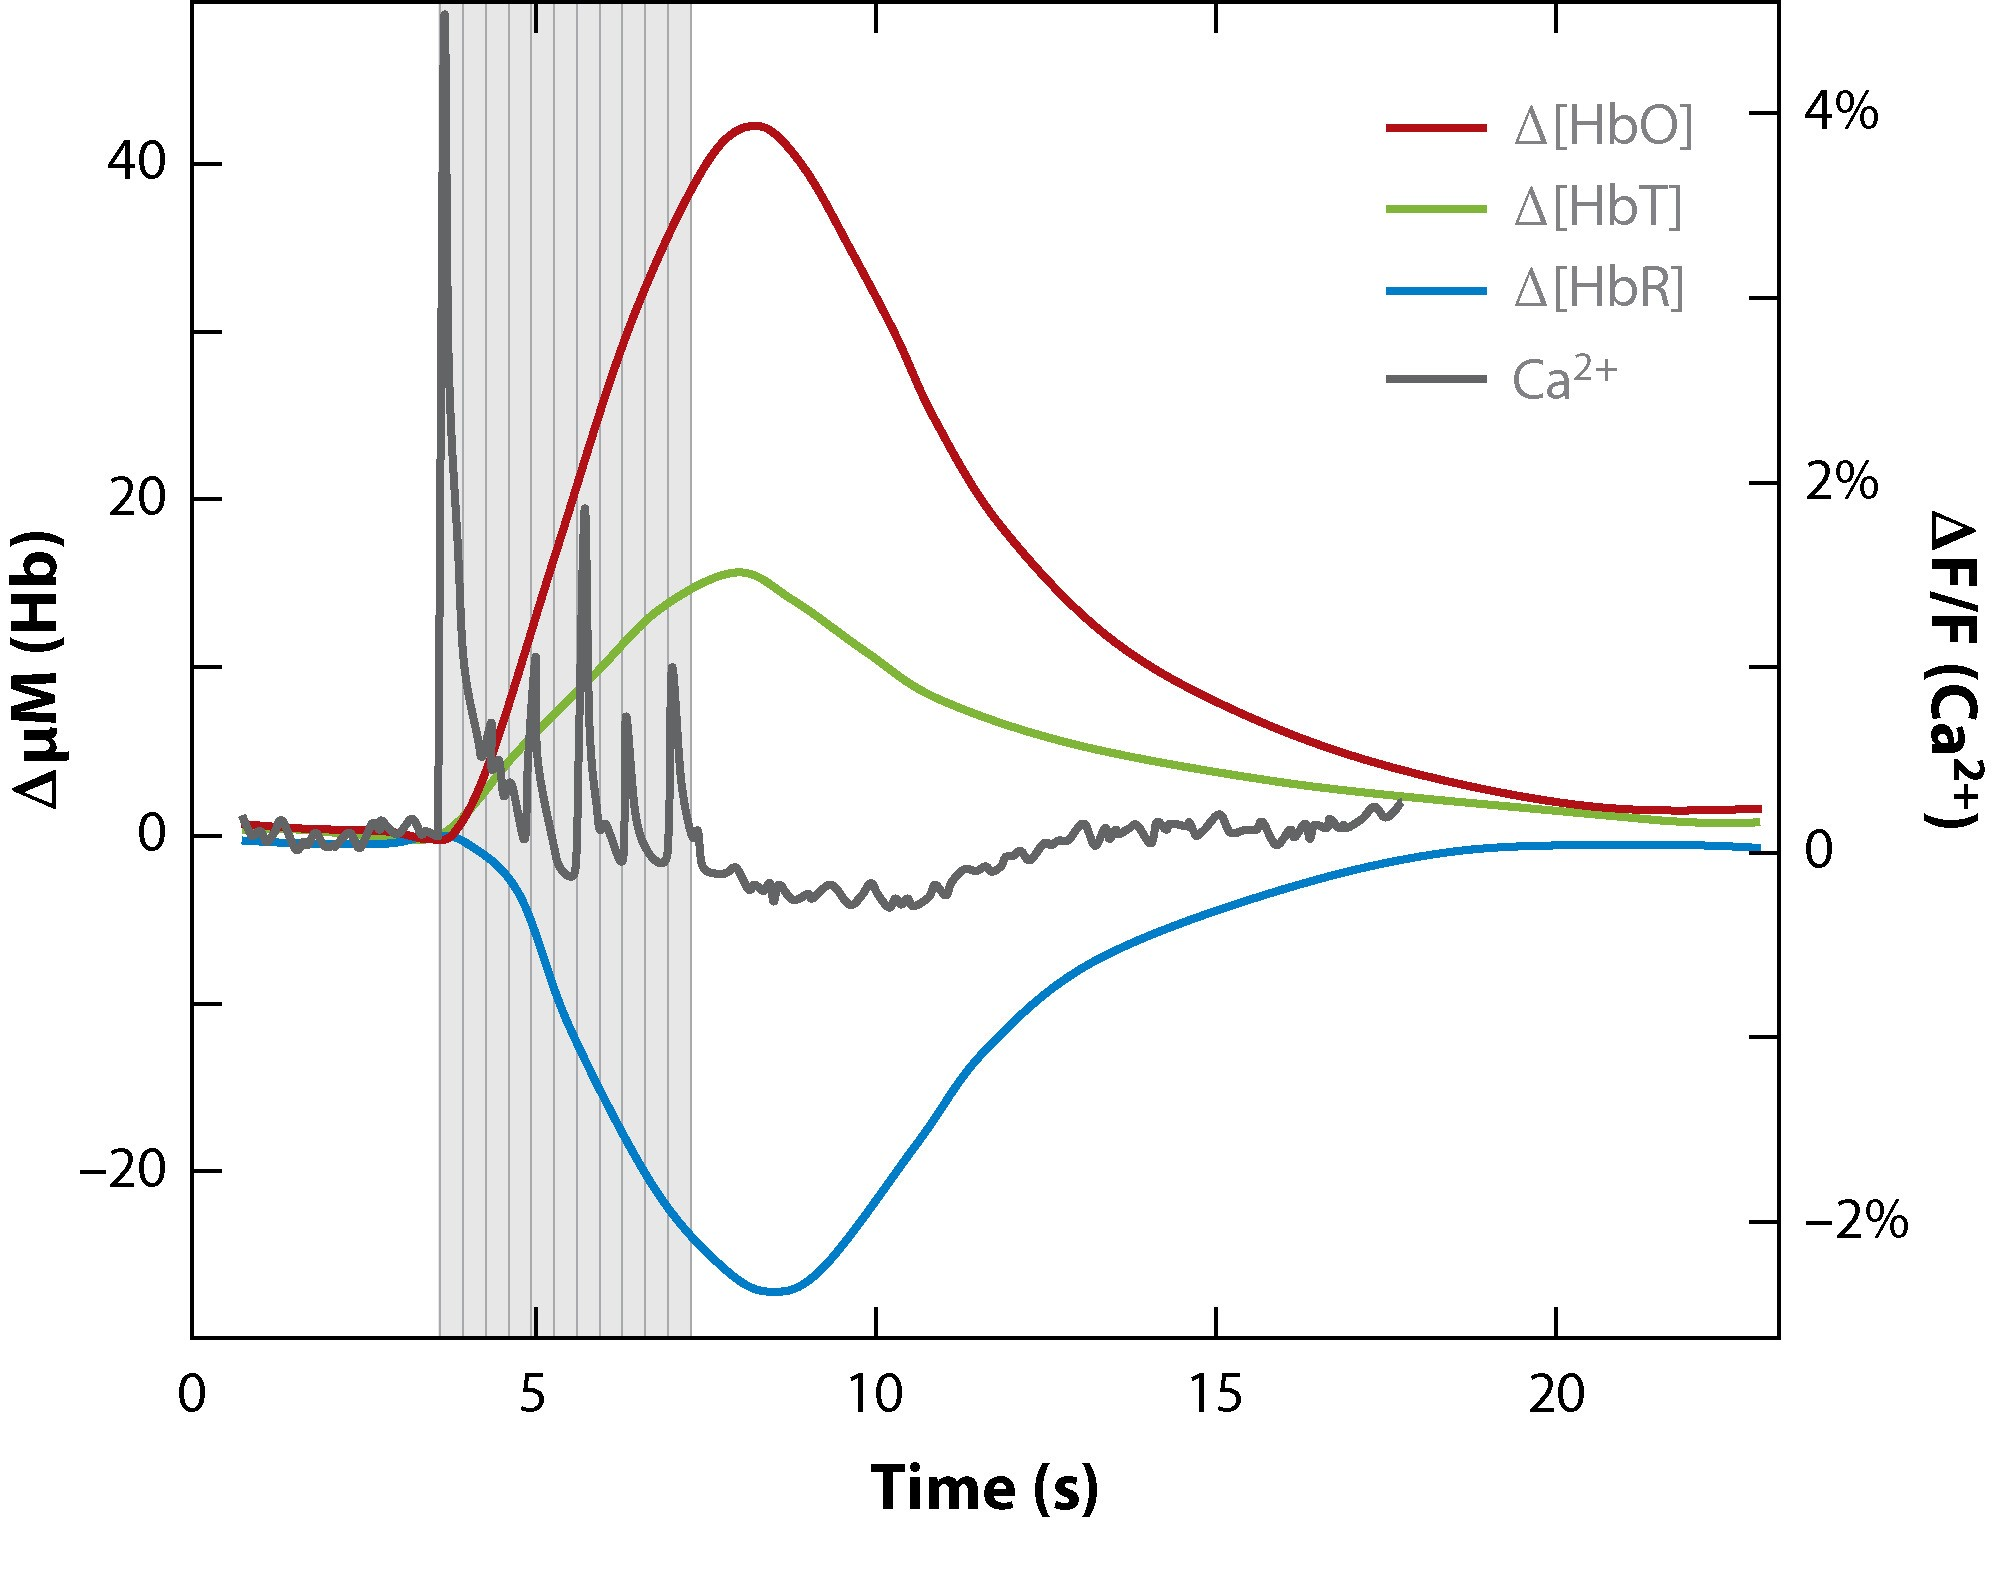
\includegraphics[width = 0.75\textwidth, height = 7cm]{assets/images/Hb_flactuations_BOLD.jpg}
    \caption[Stimulus-evoked response in somatosensory cortex of rats]{Stimulus-evoked response in somatosensory cortex of rats. Noteably, there is a distinct increase in \gls{HbT} corresponding to vessel dilation and an increase in the number of red blood cells per unit volume of cortex, consistent with an increase in blood flow. \gls{HbO} increases while \gls{HbR} decreases, indicating a net overoxygenation of the region. The \gls{fMRI} \gls{BOLD} is sensitive to changes in \gls{HbR}, where stimulus-evoked "positive \gls{BOLD}" corresponds to the decrease in \gls{HbR} shown here. Adapted from Fig. 2 p.4 \paper{Hillman}{Hillman2007}.}
    \label{fig:BOLD}
\end{figure}

% Broad finishing statements.
A range of cellular mechanisms, including astrocytes, pericytes, and interneurons, have been proposed to play a role in neurovascular coupling.\cite{Hillman2014}. For classical interpretation of \gls{BOLD} signals, it is assumed that neurovascular coupling is so robust that any increase in neuronal activity generates a proportional increase in local blood flow, irrespective of brain region, brain development, and pathological state \cite{Logothetis2010}.